%!TEX root = ../main.tex

\section{Why learning?}
\begin{frame}
	\frametitle{Table of Contents}
	\tableofcontents[currentsection,currentsubsection]
\end{frame}

\begin{frame}[label=definition] 
	\begin{block}{Definitions\footnote{\citet{March1991a}}}
		\begin{enumerate}
			\item<1-> Reliability: is the learning outcome public, stable, and shared
			\item<2-> Validity: does learning aid in understanding, prediction, and control
		\end{enumerate}
	\end{block}
	\note{Humor me, please suppress your own idea of what these terms mean and work with my definition of the terms for the length of this presentation. Join me on this journey.}
\end{frame}

% Adding the number (that is higher than the count of items) removes the "multiply defined" warning and gives the frame a unique label (aparently, the number is attached to the label?). E.g.:
% \againframe<3>{definition}

\begin{frame}
	\frametitle{Learning \& Sustainability I}
	\begin{block}{Valid learning}
		Creation of quantitative/mental models that inform in advance or lead to desirable states.

		\hrulefill

		\begin{itemize}
			\item Robust climate models \citep{Manabe1967,Forster2017}
		\end{itemize}
		% \vspace{5pt}
		\centering \textbf{vs.} invalid learning
		\vspace{5pt}
		\begin{itemize}
			\item Surprising, unpredicted arctic ice loss \citep{Guarino2020}
		\end{itemize}
	\end{block}
	\note{Purpose is to convince audience that reliability \& validity are relevant to sustainability.

	Valid in what it covers, environmental impact dimension not defined.}
\end{frame}

\againframe<3>{definition}

\begin{frame}
	\frametitle{Learning \& Sustainability II}
	\begin{block}{Reliable learning}
		Developing a mental or formal model that is widely accepted.

		\hrulefill

		\begin{itemize}
			\item Collective learning process \citep{Wright2017}
			\item Bridging epistemic communities \citep{Aronczyk2019}
		\end{itemize}
		% \vspace{5pt}
		\centering \textbf{vs.} unreliable learning
		% Make it the header style
		\vspace{5pt}
		\begin{itemize}
			\item Unintentional or deliberate rejection of learning \citep{Hermwille2019,Koontz2018}
			\item Persistent resistance or ignorance \citep{Boudet2020}
		\end{itemize}
	\end{block}
	\note{Technology, pigs, real-time observation.}
\end{frame}

\blackgroup
	\begin{frame}[plain]
		What keeps valid knowledge from being reliable?
		\note{Think about reliablity \& validity as a two-by-two.

		What prevents the joint optimization of both?}
	\end{frame}
\egroup

\begin{frame}
	\frametitle{Learning \& Sustainability III}
	\begin{block}{Example of conflicts}
		\begin{itemize}
			\item Biases \citep[e.g.,][]{Makov2016}
			\item After building coalition, validity of knowledge in doubt \citep[e.g.,][]{Aronczyk2019,Wright2017}
			\item Entrenched invalid learning \citep[e.g.,][]{Boudet2020}
			\item Knowledge gap between layman and (relative) experts \citep[e.g.,][]{Camilleri2019}
			\item Self-interest \citep{Rerup2021}
		\end{itemize}
		% Self-interest
	\end{block}
	\note{
	\begin{itemize}
		\item \citetitle{Makov2016} \citep{Makov2016}
		\item \citetitle{Boudet2020} \citep{Boudet2020}
	\end{itemize}
	}
\end{frame}

\begin{frame}
	\frametitle{Example 1}
	\begin{block}{\citet{Maguire2009}}
		\begin{enumerate}
			\item <1-> 1950s: DDT is most used pesticide
			\item <2-> 1963: Rachel Carlson problematizes DDT adverse impacts in \textit{Silent Spring}
				\subitem Human health
				\subitem Environmental impact
			\item <3-> 1960s: Cost-benefit discussions in \textit{Science}, \textit{Ecology} etc.
			\item <4-> 1972: EPA investigates, bans DDT nationwide
				\subitem DDT use already down 67\%
		\end{enumerate}
	\end{block}
	\note{Let me show you how we think this works.

	Acknowledge that this is deliberately using their language.}
\end{frame}

\begin{frame}
	\begin{center}
		\frametitle{Examples}
		DDT\\
		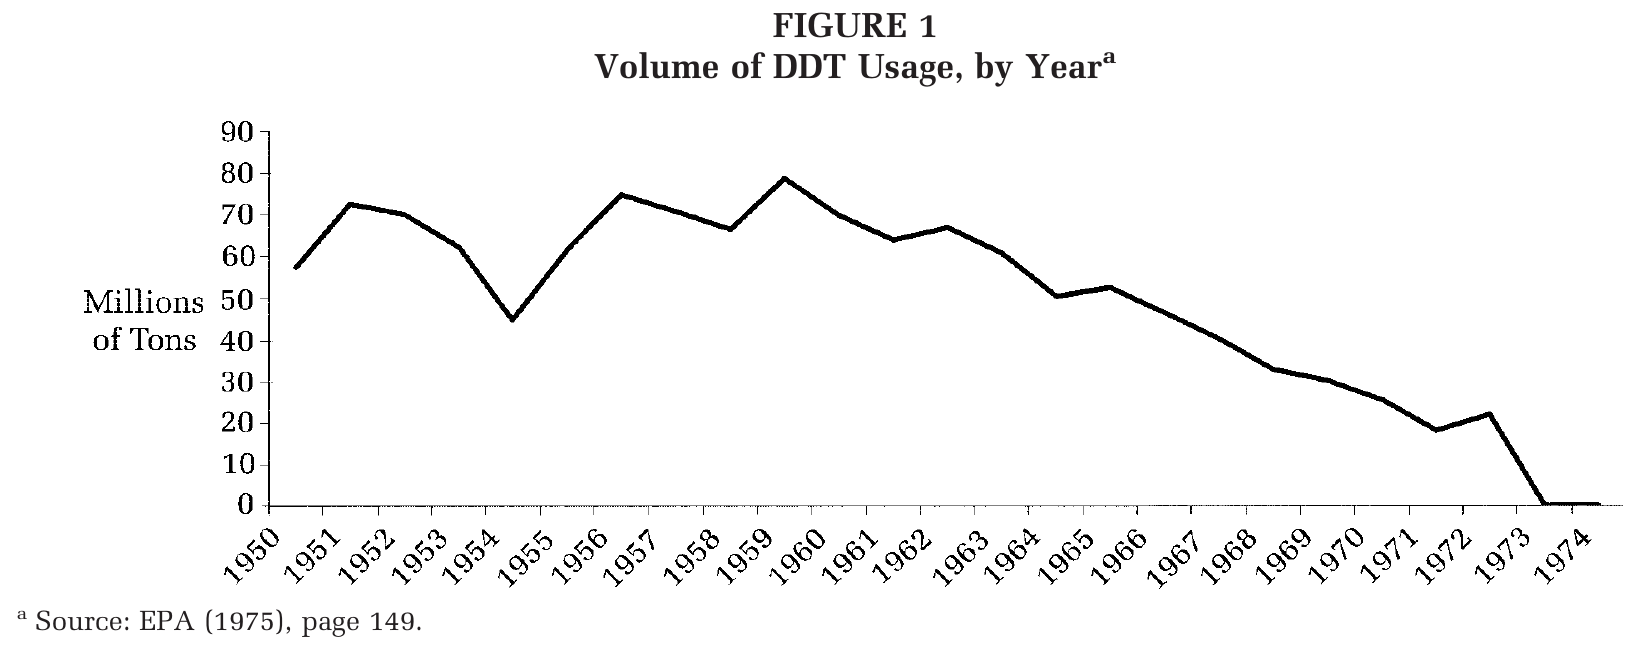
\includegraphics[width=0.7\textwidth]{illustrations/Maguire_Hardy_Fig_1.png}\\
			\textbf{vs.}\\

		Pipeline spills\\	
		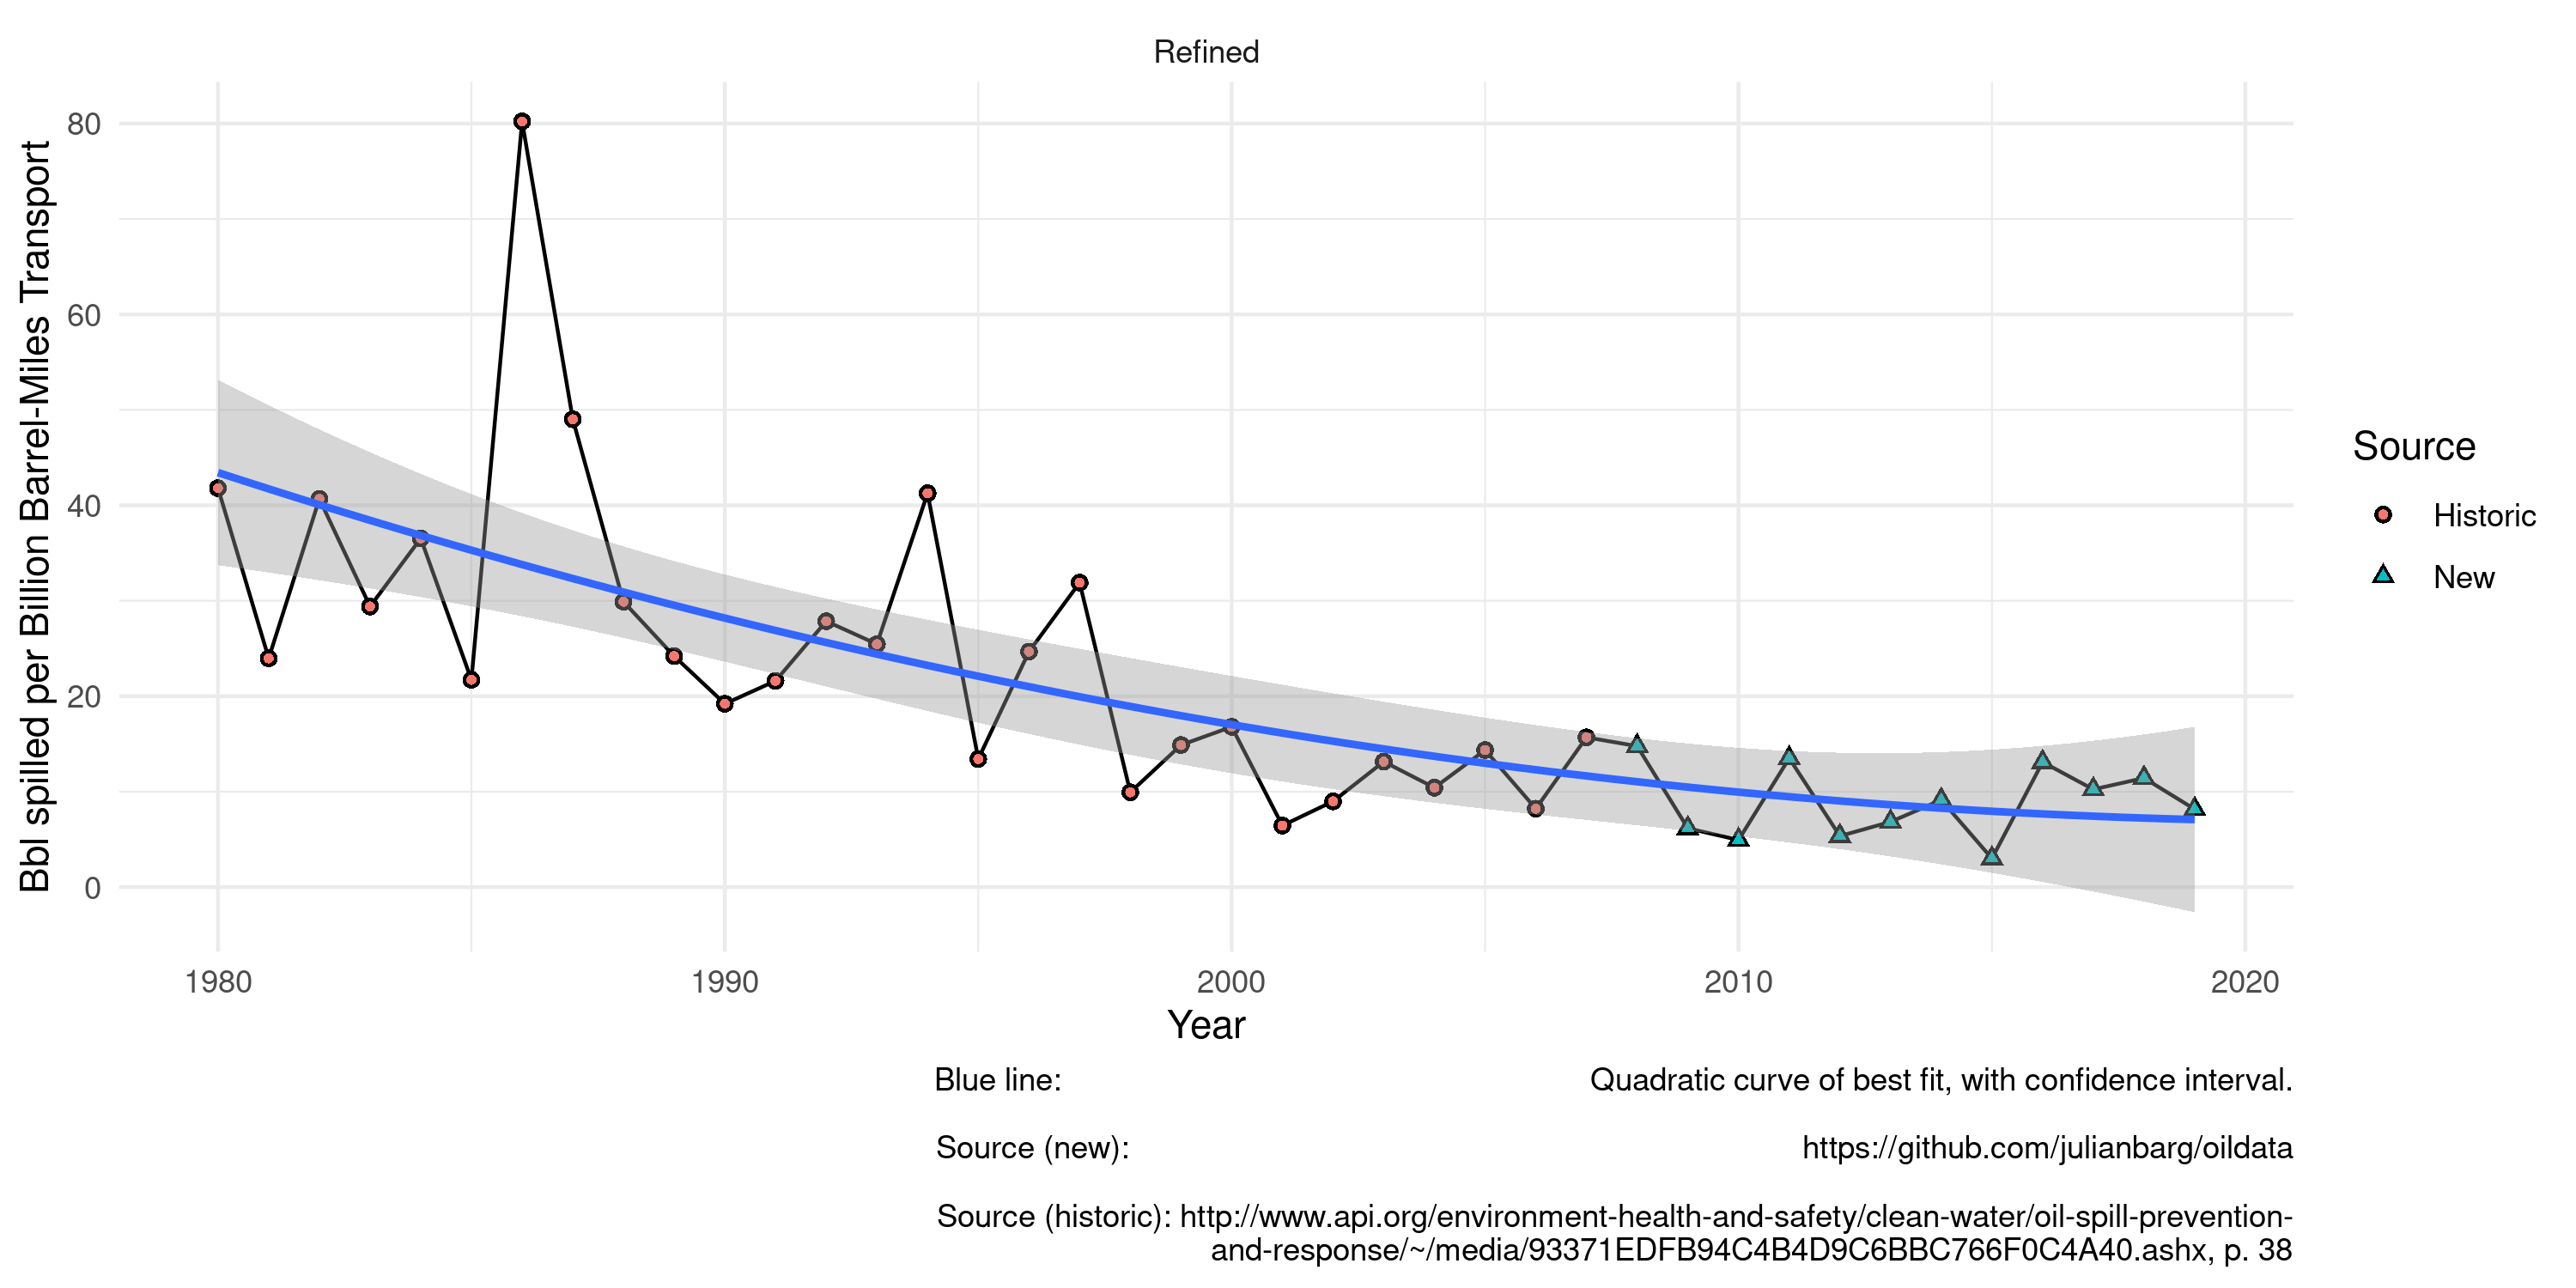
\includegraphics[width=0.7\textwidth]{illustrations/pipeline_spill_trend.png}
	\end{center}
% 	\begin{columns}[t]
% 		\begin{column}{0.48\textwidth}
% 			\# MH Figure 1
% 		\end{column}
% 		\vrule{}
% 		\begin{column}{0.48\textwidth}
% 			\# Pipeline figure 1
% 		\end{column}
% 	\end{columns}
\end{frame}

\againframe<4>{definition}

\begin{frame}
	\frametitle{Example 2}
	\begin{block}{Pipeline industry\footnote{\citet{Estes2019}}}
		\begin{enumerate}
			\item <1-> Mid-century enthusiasm for oil \& pipelines
				\subitem Consensus--engineering epistemology reliable \& valid
			\item <2-> Problematization
				\subitem Prominent spills (e.g., Exxon Valdez)
				\subitem Environmental movement
			\item <3-> Industry offers partial response
				\subitem Pipeline safety technology
				\subitem Advertisement \& lobbying
			\item <4-> Tension persists
				\subitem Coexistence of two epistemic communities
				\subitem Limited communication
		\end{enumerate}
	\end{block}
	\note{
		\begin{itemize}
			\item Mid-century: wave of infrastructure building into 60s \& 70s
			\item Exxon Valdez led to coalescence of resistance
			\item Example standing rock, water warriors
			\item At the end, no new valid and reliable understanding
		\end{itemize}
	}
\end{frame}

\blackgroup
\begin{frame}[plain]
	% Purpose I
	\note{
		\begin{itemize}
			\item You can see how the concepts are useful?
			\item Useful concepts to describe phenomena in sustainability.
			\item The interaction of physical \& social world makes them important here.
				\subitem Great insights into pollution and climate change
				\subitem Limited dissemination
		\end{itemize}

		\hrulefill

		The first thing I am working on is to explore reliability \& validity by its own right. Without focus on pipeline data.
	}
\end{frame}
\egroup
